\section{Implémentation et tests}

Le but de ce travail était tout d'abord d'implémenter la méthode décrite dans l'article \cite{farbman2011tonal}, puis dans un second temps d'évaluer la méthode sur un certain nombre de jeux d'exemples. 

\subsection{Validation de la méthode de Nystrom pour l'évaluation de W}
Afin d'implémenter la méthode décrite dans \cite{farbman2011tonal}, il a tout d'abord fallu implémenter la méthode de Nystrom pour estimer une approximation de la matrice de similarité W.

Afin de valider l'algorithme, une image de petite taille en niveau de gris synthétique a été créée (voir image \ref{nystrom_synth}).

\begin{figure}[h]
\centering

\includegraphics[width=0.2\textwidth]{Chapters/Images/nystrom_synthetic}
\caption{Image synthétique en niveau de gris de taille $10\times 10$}
\label{nystrom_synth}
\end{figure}

Le but de la validation est de comparer la véritable matrice de similarité W avec l'approximation obtenue avec la méthode de Nystrom. La figure \ref{fig_nystrom_results} compare la matrice de similarité réelle avec une approximation à 1, 3, 5, 7, et 9 vecteurs propres. On peut observer que l'on arrive à une approximation de $W_{reel}$ sans avoir besoin de beaucoup de valeur et vecteurs propres. La figure \ref{fig_rms} représente l'évolution de la RMSE selon le nombre de valeurs propres choisies.

\begin{figure}[H]
\centering
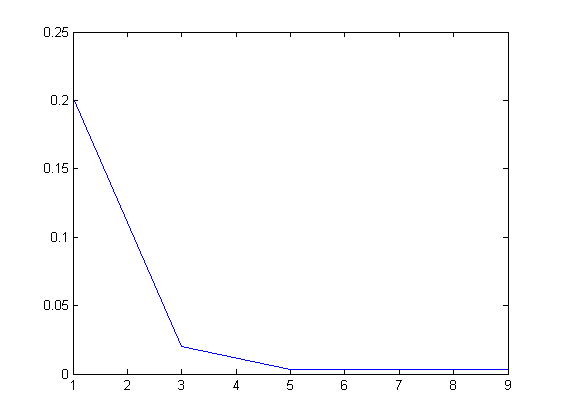
\includegraphics[width = 0.5\textwidth]{Chapters/Images/rms}
\caption{RMSE en fonction du nombre de valeur propres pour l'estimation de $W$}
\label{fig_rms}
\end{figure}

\begin{figure}[H]
\centering
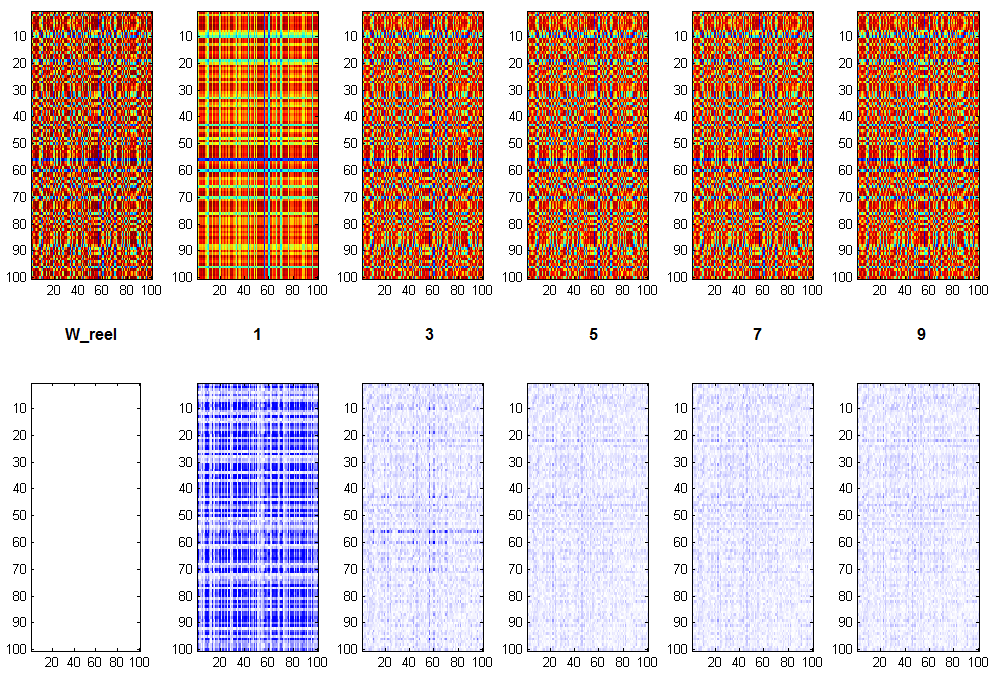
\includegraphics[width =\textwidth]{Chapters/Images/eigenvalues}
\caption{Haut : Carte de similarité $W$, et $\tilde{W}_{n}$ (approximation de $W$ à la n\up{ème} valeur propre). Bas : Erreur par rapport à $W_{reel}$}
\label{fig_nystrom_results}
\end{figure}


\subsection{Tests de stabilisation tonale}
Les séquences vidéos présentées dans l'article \cite{farbman2011tonal} sont disponible en téléchargement. Ces données ont donc été utilisées afin de réaliser les tests.\\

Tout d'abord, la séquence initiale \textit{graycard.avi} a été alignée afin de conserver une tonalité froide (figure \ref{fig_gray}), puis sur une tonalité chaude.

\begin{figure}[H]
\begin{tabular}{ccccc}
\includegraphics[width = 0.2\textwidth]{Chapters/Images/Seq_init/1}&
\includegraphics[width = 0.2\textwidth]{Chapters/Images/Seq_init/2}&
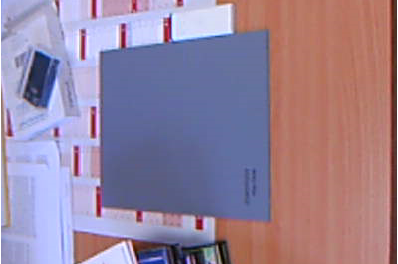
\includegraphics[width = 0.2\textwidth]{Chapters/Images/Seq_init/3}&
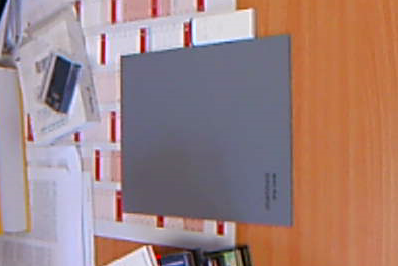
\includegraphics[width = 0.2\textwidth]{Chapters/Images/Seq_init/4}&
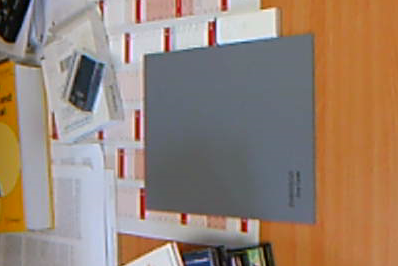
\includegraphics[width = 0.2\textwidth]{Chapters/Images/Seq_init/5}\\

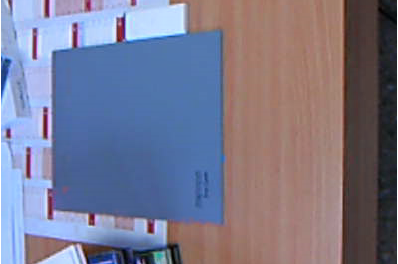
\includegraphics[width = 0.2\textwidth]{Chapters/Images/Seq_cold/1}&
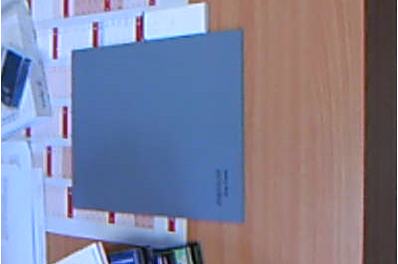
\includegraphics[width = 0.2\textwidth]{Chapters/Images/Seq_cold/2}&
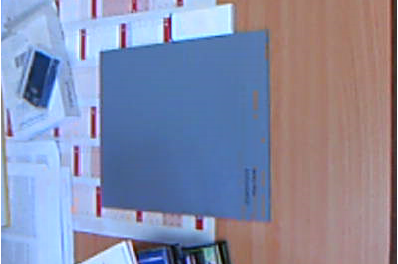
\includegraphics[width = 0.2\textwidth]{Chapters/Images/Seq_cold/3}&
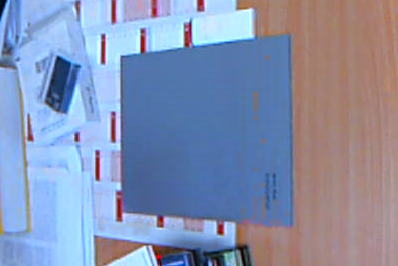
\includegraphics[width = 0.2\textwidth]{Chapters/Images/Seq_cold/4}&
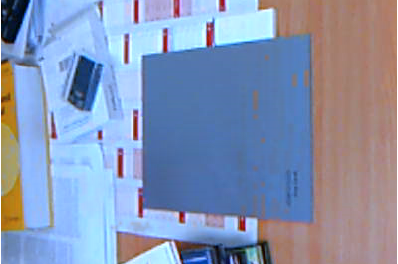
\includegraphics[width = 0.2\textwidth]{Chapters/Images/Seq_cold/5}\\

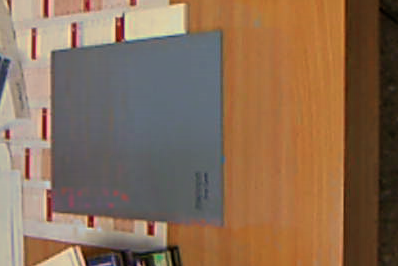
\includegraphics[width = 0.2\textwidth]{Chapters/Images/Seq_warm/1}&
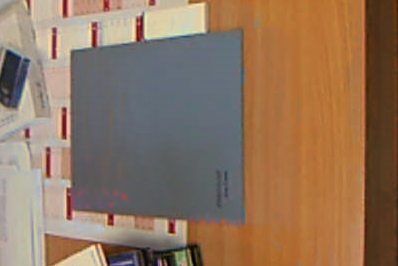
\includegraphics[width = 0.2\textwidth]{Chapters/Images/Seq_warm/2}&
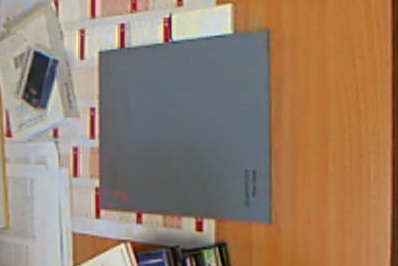
\includegraphics[width = 0.2\textwidth]{Chapters/Images/Seq_warm/3}&
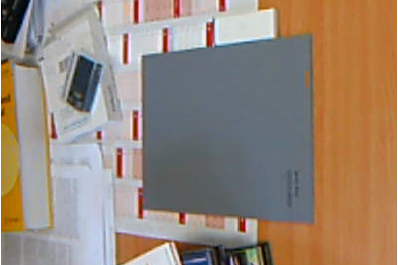
\includegraphics[width = 0.2\textwidth]{Chapters/Images/Seq_warm/4}&
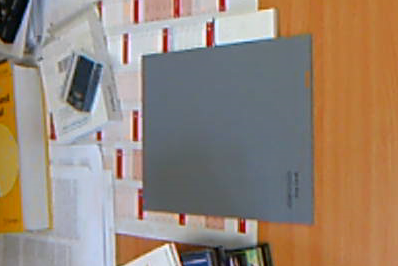
\includegraphics[width = 0.2\textwidth]{Chapters/Images/Seq_warm/5}
\end{tabular}
\caption{Haut : Séquence initiale, Milieu : Séquence alignée sur la première image, Bas : Séquence alignée sur la dernière image. Les images sont prises à 10 images d'intervalle par rapport à la séquence complète.}
\label{fig_gray}
\end{figure}

On peut voir sur la figure \ref{fig_gray} que l'on a effectivement réussi à stabiliser les fluctuations tonales de la vidéo autour. On note tout de même quelques artéfacts de couleur sur l'image.\\

On peut cependant se poser la question de l'impact de l'algorithme de stabilisation tonale sur une séquence pendant laquelle le changement d'illumination ne serait pas dû à une correction de l'appareil photo mais à une baisse ou une hausse de luminosité naturelle de la scène. L'image \ref{fig_illum} montre le résultat d'une séquence dans laquelle la lumière a été baissé progressivement, et la stabilisation de la séquence sur une image sombre. \\


\begin{figure}[H]
\begin{tabular}{ccccc}
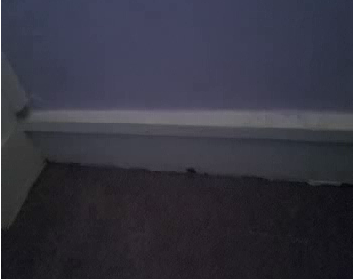
\includegraphics[width = 0.2\textwidth]{Chapters/Images/Seq_ill/2}&
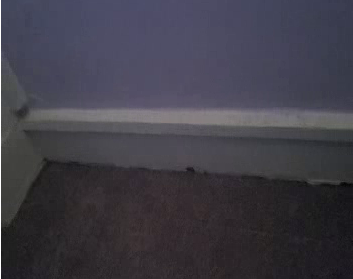
\includegraphics[width = 0.2\textwidth]{Chapters/Images/Seq_ill/3}&
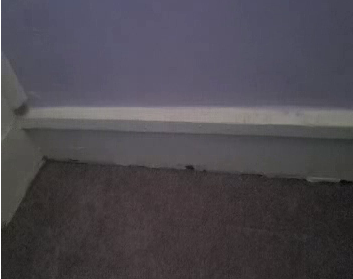
\includegraphics[width = 0.2\textwidth]{Chapters/Images/Seq_ill/4}&
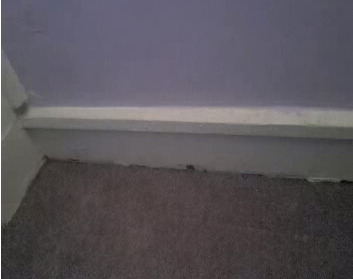
\includegraphics[width = 0.2\textwidth]{Chapters/Images/Seq_ill/5}&
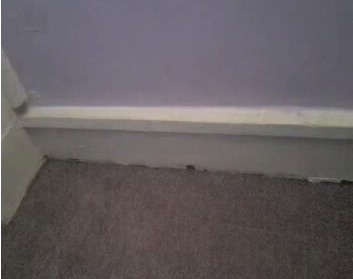
\includegraphics[width = 0.2\textwidth]{Chapters/Images/Seq_ill/6}\\

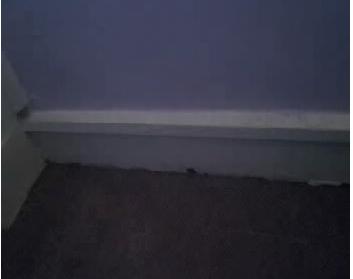
\includegraphics[width = 0.2\textwidth]{Chapters/Images/Seq_ill_stab/2}&
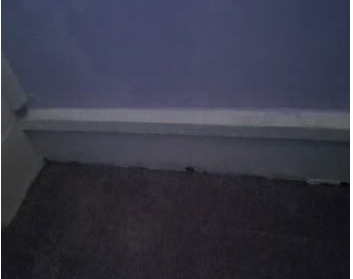
\includegraphics[width = 0.2\textwidth]{Chapters/Images/Seq_ill_stab/3}&
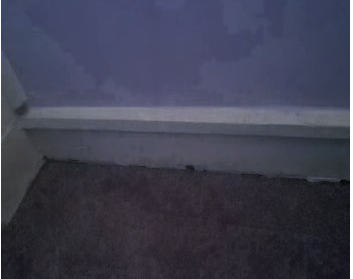
\includegraphics[width = 0.2\textwidth]{Chapters/Images/Seq_ill_stab/4}&
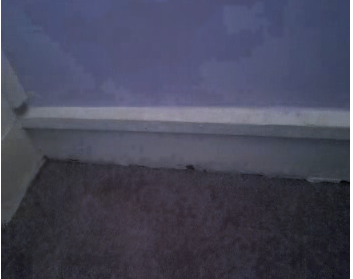
\includegraphics[width = 0.2\textwidth]{Chapters/Images/Seq_ill_stab/5}&
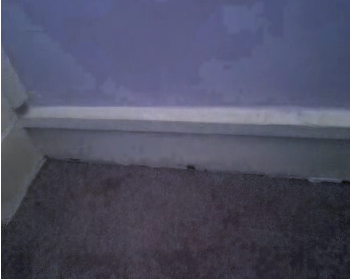
\includegraphics[width = 0.2\textwidth]{Chapters/Images/Seq_ill_stab/6}

\end{tabular}
\caption{Haut : Séquence initiale, Bas : Séquence alignée sur la première image}
\label{fig_illum}
\end{figure}


On peut tout d'abord noter que la séquence a été stabilisée alors qu'aucune correction n'avait été apporté par l'appareil. D'autre part, on note la présence d'artéfacts sur l'image. Ces artéfacts ont plusieurs origines. Tout d'abord, les images ont été sous-échantillonnés pour le calcul des cartes d'ajustements et le nombre de pixels est donc très bas. D'autre part, dans des conditions de très basse lumière comme celle-ci, les images ne sont pas nettes.\\

Enfin, un test a été réalisé afin d'observer le comportement de l'algorithme en regard de la cohérence temporelle de la séquence d'image. Afin de réalisée ce test, deux bout de séquences ont été concaténées afin de créer une coupure artificielle de la vidéo. On peut remarquer sur l'image \ref{fig_coherence} que la perte de cohérence temporelle influe énormément sur le résultat de l'algorithme.

\begin{figure}[H]
\begin{tabular}{ccccc}
\includegraphics[width = 0.2\textwidth]{Chapters/Images/Seq_temp/1}&
\includegraphics[width = 0.2\textwidth]{Chapters/Images/Seq_temp/2}&
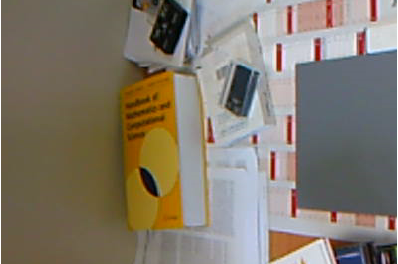
\includegraphics[width = 0.2\textwidth]{Chapters/Images/Seq_temp/3}&
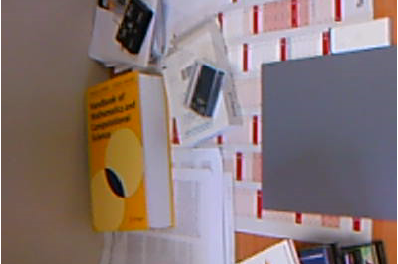
\includegraphics[width = 0.2\textwidth]{Chapters/Images/Seq_temp/4}&
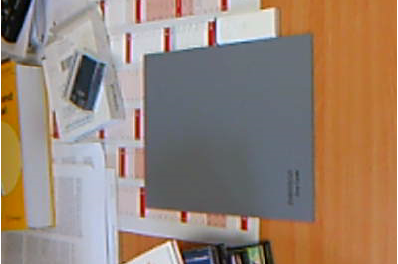
\includegraphics[width = 0.2\textwidth]{Chapters/Images/Seq_temp/5}\\

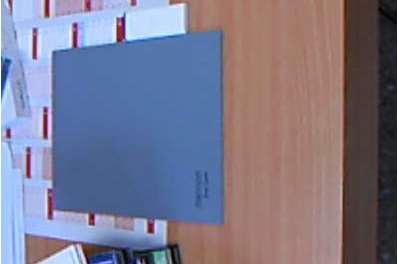
\includegraphics[width = 0.2\textwidth]{Chapters/Images/Seq_temp_stab/1}&
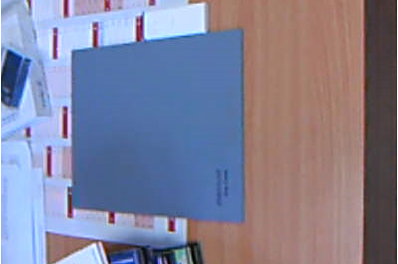
\includegraphics[width = 0.2\textwidth]{Chapters/Images/Seq_temp_stab/2}&
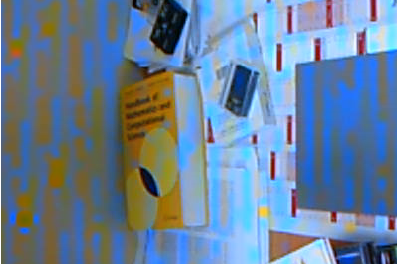
\includegraphics[width = 0.2\textwidth]{Chapters/Images/Seq_temp_stab/3}&
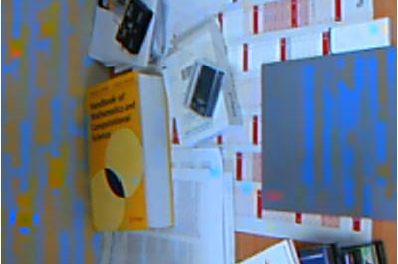
\includegraphics[width = 0.2\textwidth]{Chapters/Images/Seq_temp_stab/4}&
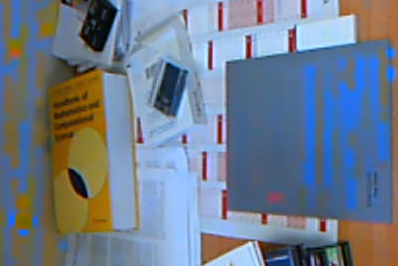
\includegraphics[width = 0.2\textwidth]{Chapters/Images/Seq_temp_stab/5}

\end{tabular}
\caption{Haut : Séquence initiale, perte de cohérence temporelle, Bas : Séquence alignée sur la première image}
\label{fig_coherence}
\end{figure}

